\documentclass[border=12pt]{standalone}
\usepackage{tikz}
\usetikzlibrary{shapes.geometric, arrows.meta, positioning, calc, fit, backgrounds}
\usepackage{fontspec}
\usepackage{amsmath,amssymb}
\setmainfont{DejaVu Sans}

\begin{document}
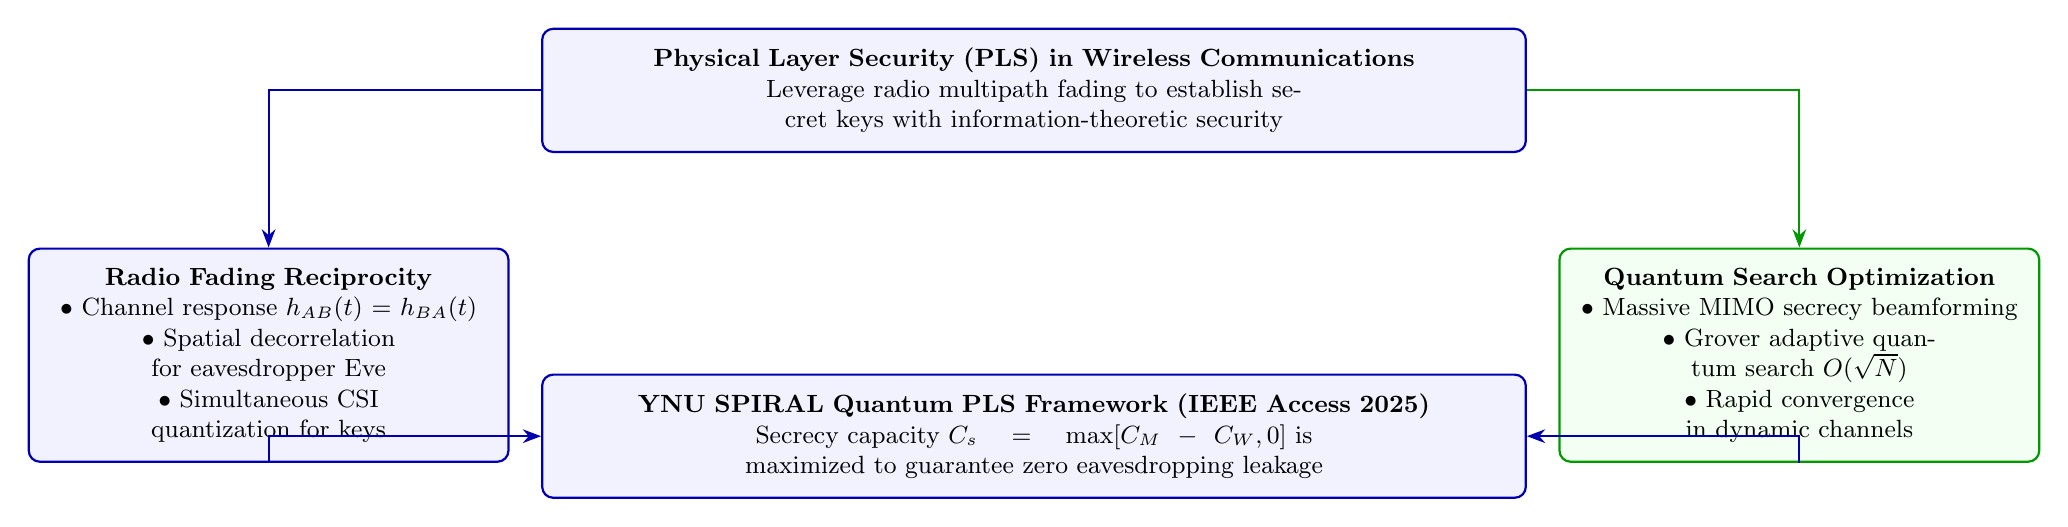
\begin{tikzpicture}[
    font=\small,
    >=Stealth,
    node distance=1.2cm,
    block/.style={rectangle, draw=blue!70!black, fill=blue!5, rounded corners=4pt, thick, align=center, inner sep=7pt},
    alertblock/.style={rectangle, draw=red!70!black, fill=red!5, rounded corners=4pt, thick, align=center, inner sep=7pt},
    greenblock/.style={rectangle, draw=green!60!black, fill=green!5, rounded corners=4pt, thick, align=center, inner sep=7pt},
    amberblock/.style={rectangle, draw=orange!80!black, fill=orange!5, rounded corners=4pt, thick, align=center, inner sep=7pt}
]

\node[block, text width=12cm] (top) {\textbf{Physical Layer Security (PLS) in Wireless Communications}\\Leverage radio multipath fading to establish secret keys with information-theoretic security};

\node[block, below left=1.2cm and 0.4cm of top, text width=5.6cm] (channel) {\textbf{Radio Fading Reciprocity}\\$\bullet$ Channel response $h_{AB}(t) = h_{BA}(t)$\\$\bullet$ Spatial decorrelation for eavesdropper Eve\\$\bullet$ Simultaneous CSI quantization for keys};

\node[greenblock, below right=1.2cm and 0.4cm of top, text width=5.6cm] (quantum) {\textbf{Quantum Search Optimization}\\$\bullet$ Massive MIMO secrecy beamforming\\$\bullet$ Grover adaptive quantum search $O(\sqrt{N})$\\$\bullet$ Rapid convergence in dynamic channels};

\node[block, below=2.8cm of top, text width=12cm] (bottom) {\textbf{YNU SPIRAL Quantum PLS Framework (IEEE Access 2025)}\\Secrecy capacity $C_s = \max [C_M - C_W, 0]$ is maximized to guarantee zero eavesdropping leakage};

\draw[->, thick, blue!70!black] (top) -| (channel);
\draw[->, thick, green!60!black] (top) -| (quantum);
\draw[->, thick, blue!70!black] (channel) |- (bottom);
\draw[->, thick, blue!70!black] (quantum) |- (bottom);

\end{tikzpicture}
\end{document}
